%\documentclass[aspectratio=169, handout]{beamer}
\documentclass[aspectratio=169]{beamer}


\makeatletter
\renewcommand*\env@matrix[1][\arraystretch]{%
  \edef\arraystretch{#1}%
  \hskip -\arraycolsep
  \let\@ifnextchar\new@ifnextchar
  \array{*\c@MaxMatrixCols c}}
\makeatother

\usepackage{tikz}
\usetikzlibrary{tikzmark,fit,shapes.geometric}

\newcommand{\transp}{^{\rm{T}}}

\usepackage{cases}
\usepackage[english]{babel}
% or whatever
\usepackage{xcolor}
\usepackage{colortbl}
\usepackage[latin1]{inputenc}
\usepackage[super]{nth}
% or whatever
%\setbeamertemplate{footline}[page number]
\setbeamertemplate{footline}
        {
      \leavevmode%
      \hbox{%
      \begin{beamercolorbox}[wd=.333333\paperwidth,ht=2.25ex,dp=1ex,center]{author in head/foot}%
        \usebeamerfont{author in head/foot}\insertshortauthor%~~(\insertshortinstitute)
      \end{beamercolorbox}%
      \begin{beamercolorbox}[wd=.333333\paperwidth,ht=2.25ex,dp=1ex,center]{title in head/foot}%
        \usebeamerfont{title in head/foot}\insertshorttitle
      \end{beamercolorbox}%
      \begin{beamercolorbox}[wd=.333333\paperwidth,ht=2.25ex,dp=1ex,right]{date in head/foot}%
        \usebeamerfont{date in head/foot}\insertshortdate{}\hspace*{2em} \insertframenumber{}  \hspace*{2em}%/ \inserttotalframenumber\hspace*{2ex} 

    %#turning the next line into a comment, erases the frame numbers
        

      \end{beamercolorbox}}%
      \vskip 0pt%
    }

\usepackage{times}
\usepackage[T1]{fontenc}
\usepackage{psfrag}
\usepackage{algorithm}
\usepackage{amsmath}
\usepackage{amssymb}
\usepackage{tabularx}
\usepackage{algpseudocode}
\usepackage{mathrsfs}
\usepackage{textpos}
\usepackage{graphicx}
\usepackage{tcolorbox}
\usepackage{multicol}
\usepackage{tikz}
\usetikzlibrary{arrows.meta,shapes.arrows}
%\setkeys{Gin}{draft}
\usepackage{caption}
\captionsetup{font=scriptsize,labelfont=scriptsize}
\usepackage{color}
\DeclareCaptionFont{blue}{\color{blue}}
\captionsetup{labelfont=blue}
\usepackage{tikz}
\tikzset{
  every overlay node/.style={
    draw=white,anchor=north west,
  },
}
\def\checkmark{\tikz\fill[scale=0.4](0,.35) -- (.25,0) -- (1,.7) -- (.25,.15) -- cycle;}
\def\tikzoverlay{%
   \tikz[baseline,overlay]\node[every overlay node]
}%
%\DeclareGraphicsRule{.png}{png}{.png.bb}{}

\newtheorem{assumption}{Assumption} %jw

\newcommand{\T}{{\rm T}}

\newcommand\blfootnote[1]{%
  \begingroup
  \renewcommand\thefootnote{}\footnote{#1}%
  \addtocounter{footnote}{-1}%
  \endgroup
}
\setcounter{tocdepth}{1}
\beamertemplatenavigationsymbolsempty


\title[Lecture 10: Multiple Regression] % (optional, use only with long paper titles)
{Data, Environment and Society: \\{Lecture 10: Multiple Regression}}


%\subtitle
%{Include Only If Paper Has a Subtitle}

\author[ER131: Data, Environment and Society] 
{Instructor: Duncan Callaway\\
GSI: Salma Elmallah} 
% - Give the names in the same order as the appear in the paper.
% - Use the \inst{?} command only if the authors have different
%   affiliation.

%\logo{
%\includegraphics[width=1.5cm,height=1.5cm,keepaspectratio]{uvic_logo_h.jpg}
%}
\vspace{-20mm}
\institute[UC Berkeley] % (optional, but mostly needed)
 {\small{ \bf October 1, 2019}}


\date[October 1, 2019]


\begin{document}

\begin{frame}[plain, noframenumbering]
  \titlepage
\end{frame}

\begin{frame}{Announcements}

\textbf{Today}
\begin{itemize}
\item First: slides, covering multiple regression and (one form of) model selection.  Slides in GitHub
\item Second: Start working with NO2 data in Jupyter notebook
\item Third: Group discussion for Alstone et al
\end{itemize}

\textbf{Reading}
\begin{itemize}
\item Next tuesday: Novotny \textit{et al}, see questions in GitHub folder for lecture 12 reading.
\item Next week: ISLR Ch 3.3.
\end{itemize}

\textbf{Survey posted!  Please respond}
\end{frame}


\begin{frame}{Mid term}

\textbf{Not intended to be hard.  }
\begin{itemize}
\item Some basic theory, formula recall and application of mathematical concepts
\begin{itemize}
\item Anything on slides or in labs
\item ISLR will reinforce, but I won't test things from ISLR not covered in lecture of lab.
\end{itemize}
\item Principles of EDA and visualization
\item Basic questions about working in Python
\begin{itemize}
\item Setting up libraries
\item Accessing information from data frames
\item Etc.  
\end{itemize}
\end{itemize}

\end{frame}

\begin{frame}{Final project}

\begin{itemize}
\item You can work with your own data
\item But we will also suggest data sets
\item Working in groups up to three ok but not required (you can self-organize)
\item We will give you basic guardrails on what to do
\begin{itemize}
\item Pose a coherent question that can be addressed using the skills we are learning
\item EDA and visualization requirements
\item Carry out multiple prediction exercises using the tools we are learning.
\item Critique the performance of your models
\item Interpret your results within the confines of what your models are capable of.
\end{itemize}
\end{itemize}

\end{frame}

\begin{frame}{What if the confidence interval contains zero?}

For example, if
   
\begin{align*}
  -10.3 < \beta_1 < 24.8?
\end{align*}

...where the upper and lower bounds comprise the 95\% confidence interval.

\pause

\vspace{5mm}
This implies there is more than a remote chance that there is no significant relationship between the dependent and independent variables.  

\end{frame}

%%%%%%%%%%%%%
\begin{frame}{p-values}

p-values measure the probability that the estimated coefficients arose by chance from a data generating process that actually has \textit{no} relationship between the inputs and outputs.  

\vspace{5mm}

$p = 0.05$ implies a 5\% chance that the true parameter value is \textit{zero}.  

\vspace{5mm}

If $p\ll0.05$, then the parameter is strongly inside the 95\% confidence interval.

\vspace{5mm}

If $p>0.05$, then the parameter is outside the 95\% confidence interval.

\vspace{5mm}

A small p-value indicates that it is unlikely to observe such a substantial association between the predictor and the response due to chance.

\end{frame}

%%%%%%%%%%%%%
\begin{frame}{p-hacking?}

What's wrong with these practices:
\begin{itemize}
  \item Stop collecting data once $p<0.05$
  \item Analyze many independent variables, but only report those for which $p<0.05$
  \item Collect and analyze many data samples, but only report those with $p<0.05$
  \item Exclude participants to get  $p<0.05$.
  \item Transform the data to get  $p<0.05$.
\end{itemize}

(credit to Leif Nelson, UCB Haas)

\end{frame}

%%%%%%%%%%%%%
\begin{frame}{The trouble with p-hacking...}

...is that by looking for the data set and the models that give low p-values, you could just be looking for those 5\% ``chances'' where the real relationship is non-existent.

\vspace{5mm}\pause

Some estimates suggest that this practice leads to false positive rates of 61\%!

\end{frame}


%%%%%%%%%%%%%
\begin{frame}{Model accuracy: R$^2$}

TSS = total sum of squares

\vspace{3mm}

RSS = residual sum of squares

  \begin{align*}
    R^2 = \frac{TSS - RSS}{TSS} \onslide<2->{= \frac{\sum_{i=1}^n (y_i-\bar{y})^2 - \sum_{i=1}^n e_i^2}{\sum_{i=1}^n (y_i-\bar{y})^2}}\onslide<3->{ = 1-\frac{\sum_{i=1}^n e_i^2}{\sum_{i=1}^n (y_i-\bar{y})^2} }
  \end{align*}

  \pause\pause
  $R^2$ measures the fraction of variation in the dependent variable that is captured by the model.  

\pause
\vspace{5mm}

It's good for capturing predictive power, but not for evaluating the significance of the model.

\end{frame}

\begin{frame}{Multivariate regression}

This is exactly the same process as single (independent) variable regression.  Parameters solutions can be found by
\begin{itemize}
\item Gradient search
\item Normal equations
\item Setting partial derivatives of MSE to zero and solving -- but now for $\beta_0, \beta_1, \beta_2,\ldots,\beta_d$ ($d$ is the number of features, a.k.a. independent variables).
\end{itemize}

\vspace{5mm}
The mechanics of finding parameters is easy.  The real challenge is: Which features to include?
\end{frame}

\begin{frame}{Model selection}

\textbf{The challenge:} Don't include variables in your model that lead to over-fit.

\vspace{-5mm}

\begin{figure}
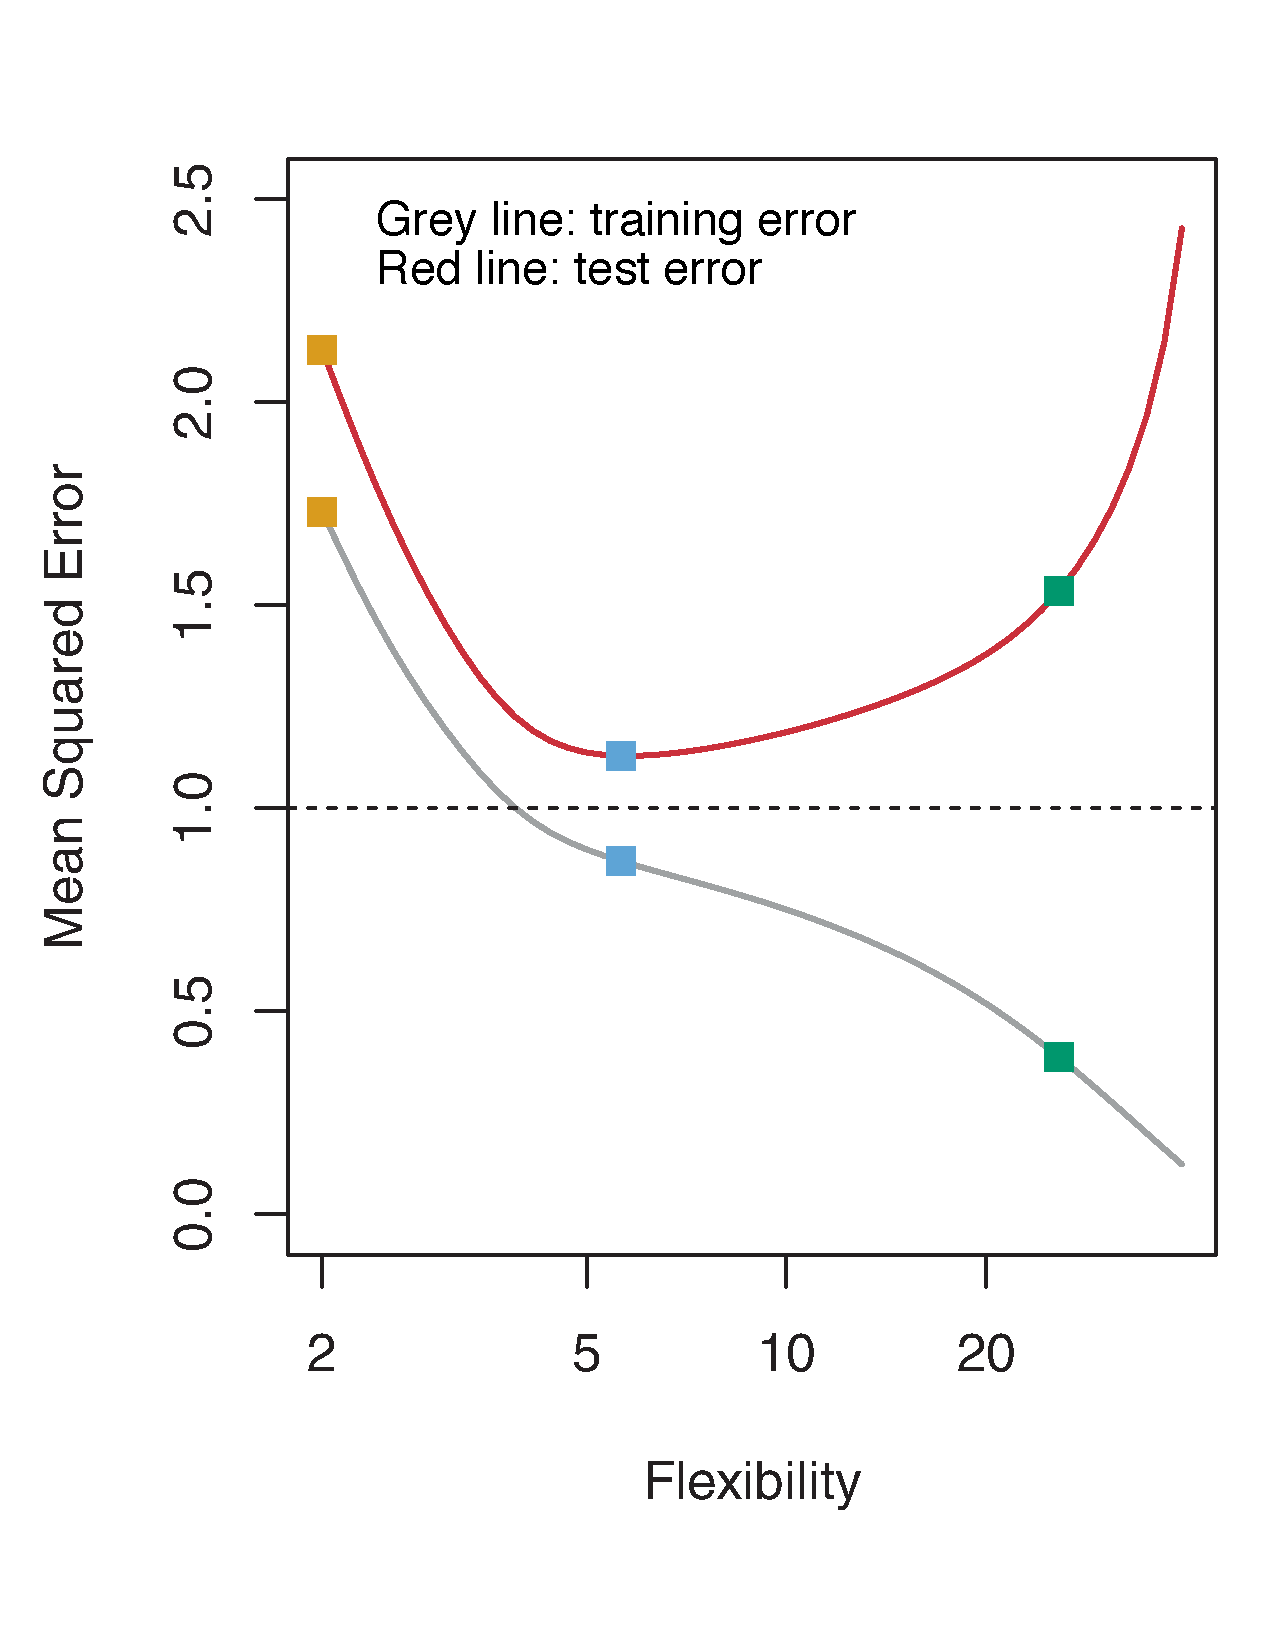
\includegraphics[height=0.8\textheight]{islr2_9b}
\end{figure}

\vspace{-10mm}
With multiple regression, increasing the number of variables increases the flexibility of the model.

\end{frame}

\begin{frame}{Model selection methods}

\textbf{Two basic methods:}
\vspace{5mm}
\begin{itemize}
\item Computationally heavy and theoretically robust: 
\begin{itemize}
\item repeated sampling of train and test data sets
\item build and test models with each sampled set
\item choose the model form that minimizes test error, on average.
\item the figure on the previous slide is an example of this approach.
\end{itemize}
\vspace{5mm}
\item Easy to implement (no need for significant computing):
\begin{itemize}
\item Use the full data set
\item Fit each candidate model once
\item Choose the model that minimizes an ``adjusted'' measure of R2 or mean squared error.
\end{itemize}
\end{itemize}
\end{frame}

\begin{frame}{An easy-to-implement method}

Akaike information criterion (AIC):

\begin{enumerate}
\item Construct all the models you have time for using \textit{all} the data to train the models.
\item Then, choose the model with the lowest AIC, where
\begin{align*}
\text{AIC} = \frac{1}{n\hat{\sigma}^2}(\text{RSS}+2d\hat{\sigma}^2) \onslide<2->{= \frac{1}{\hat{\sigma}^2}\left(\frac{\text{RSS}}{n}\right) + \frac{2d}{n}}
\end{align*}
\end{enumerate}

\pause
As you can see, AIC ``penalizes'' models with a high value of $d$.  
\end{frame}

\begin{frame}{What the heck is AIC?}

It actually has a rigorous theoretical underpinning.  Understanding the derivation requires background in information theory and more time than we have here.  

\vspace{5mm}
\pause

But:
\begin{itemize}
\item It gives unbiased estimate of the MSE you'd get if you \textit{did }use a test data set (as long as the errors are Gaussian)
\item It's ok to just work with the intuition that choosing models that minimize AIC is analogous to 
\begin{itemize}
\item choosing models that minimize MSE ...
\item plus a penalty for the number of features.
\end{itemize}
\end{itemize}

\end{frame}



\begin{frame}{Prediction application: Land use regression}
  \begin{itemize}
    \item Suppose we'd like to know pollutant concentrations at a fine spatial resolution
    \item We only have pollutant measurements at low resolution (coarse spatial scale)
    \item But we have other measurements at finer spatial resolution
    \item This is an ideal job for forecasting.  
    \item But rather than forecast in \textit{time} we will forecast in \textit{space}.
  \end{itemize}

\begin{columns}
\column{0.75\textwidth}
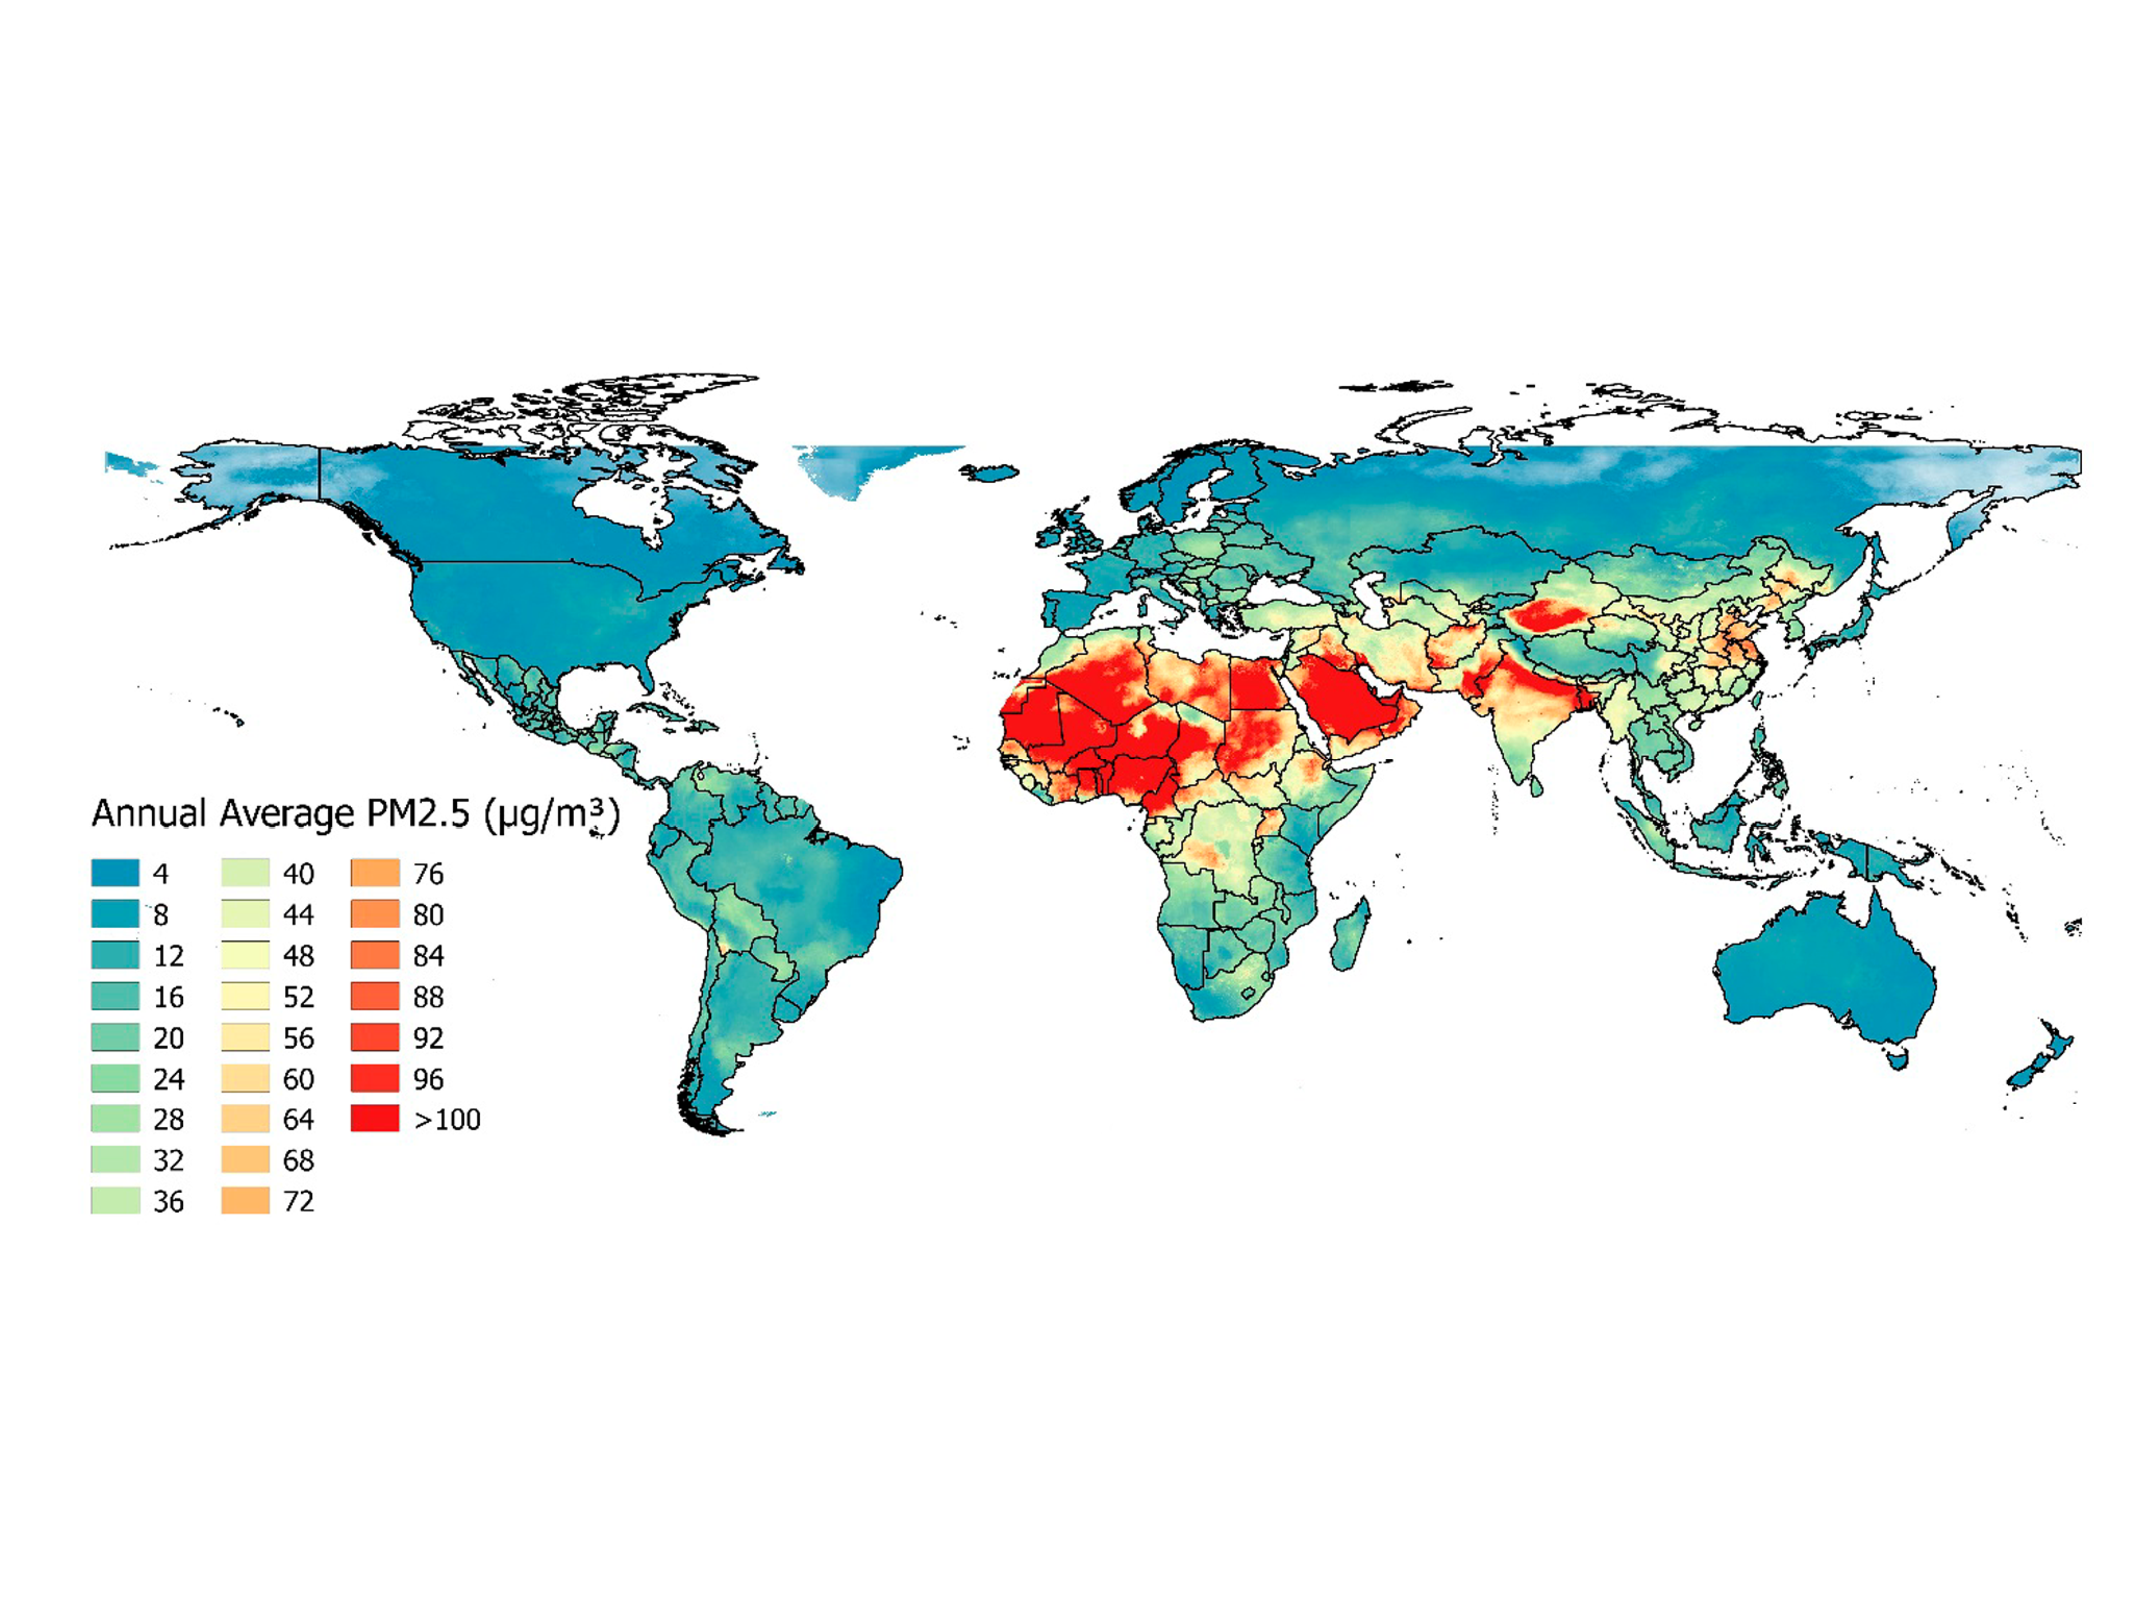
\includegraphics[width = \textwidth]{pm2_5_LUR_Shaddick.pdf}
\column{0.25\textwidth}
(From Shaddick \textit{et al} ES\&T 2018)
\end{columns}
\end{frame}

\begin{frame}{Nitrogen dioxide}

NO$_2$:
\begin{itemize}
\item Direct product of fossil fuel combustion
\item Used as an indicator for larger group of nitrogen oxides.
\item Health impact: Contributes to development of, and aggravates, asthma 
\item Environmental impact: Haze, acid rain, nutrient pollution in coastal waters
\end{itemize}

EPA Regulates NO2:
\begin{figure}
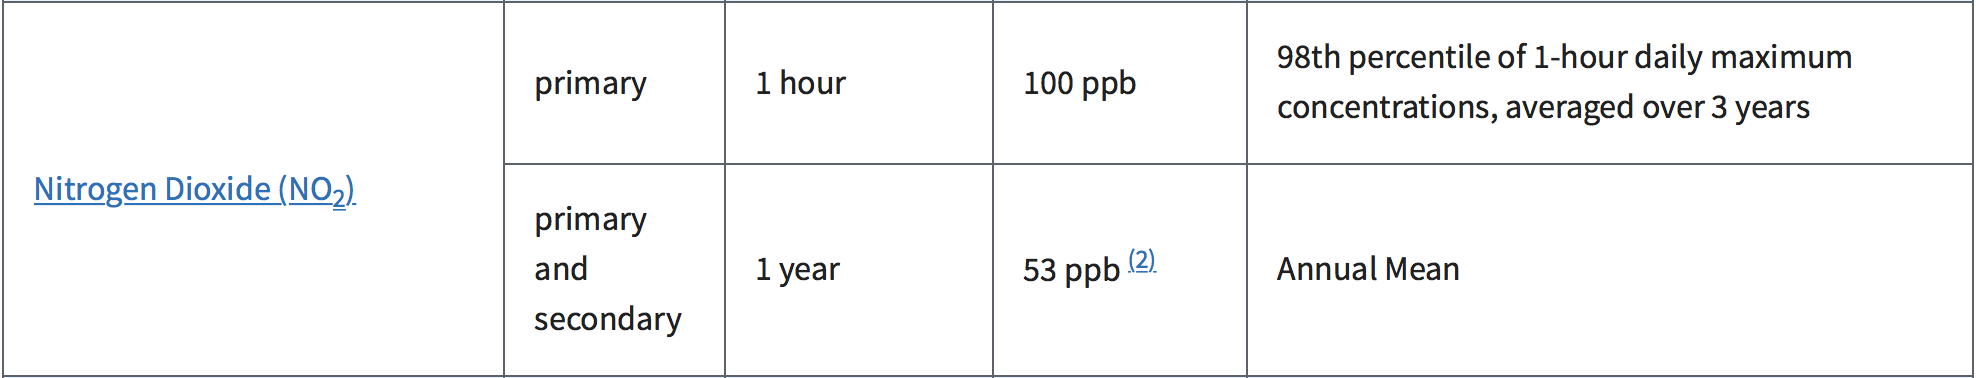
\includegraphics[width=\textwidth]{EPA_NO2_reg}
\end{figure}
\end{frame}

\begin{frame}{Novotny \textit{et al} setup}

\begin{itemize}
\item NO$_2$ concentrations are known where monitors are present.  
\item But we don't have monitors everywhere
\item Can we \textit{predict} concentrations where monitors are absent?
\end{itemize}

\pause
\begin{columns}
\column{0.5\textwidth}
\textbf{``Remote sensing'' data from satellites can be useful:}
\begin{itemize}
\item Aurora satellite ``Ozone Monitoring Instrument'' provides tropospheric NO2 column abundance (units: ppb; Called ``WRF+DOMINO'' in data set we'll work with).
\end{itemize}

\column{0.5\textwidth}
\begin{figure}
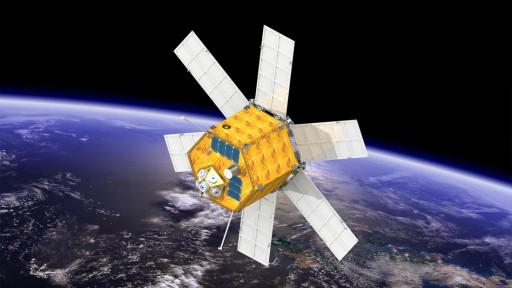
\includegraphics[width=0.75\textwidth]{aurora}
\caption*{}
\end{figure}
\end{columns}


\pause
\textbf{But!}
\begin{itemize}
\item Measurements are for entire column of air above a location, not ground-level
\item Spatial resolution is low
\end{itemize}

\end{frame}

\begin{frame}{Land use regression for NO$_2$}

\textbf{Dependent variable}: Hourly NO$_2$ concentrations from EPA sensors.

\vspace{3mm}
\textbf{Independent variables} to consider:
\vspace{-5mm}
\begin{figure}
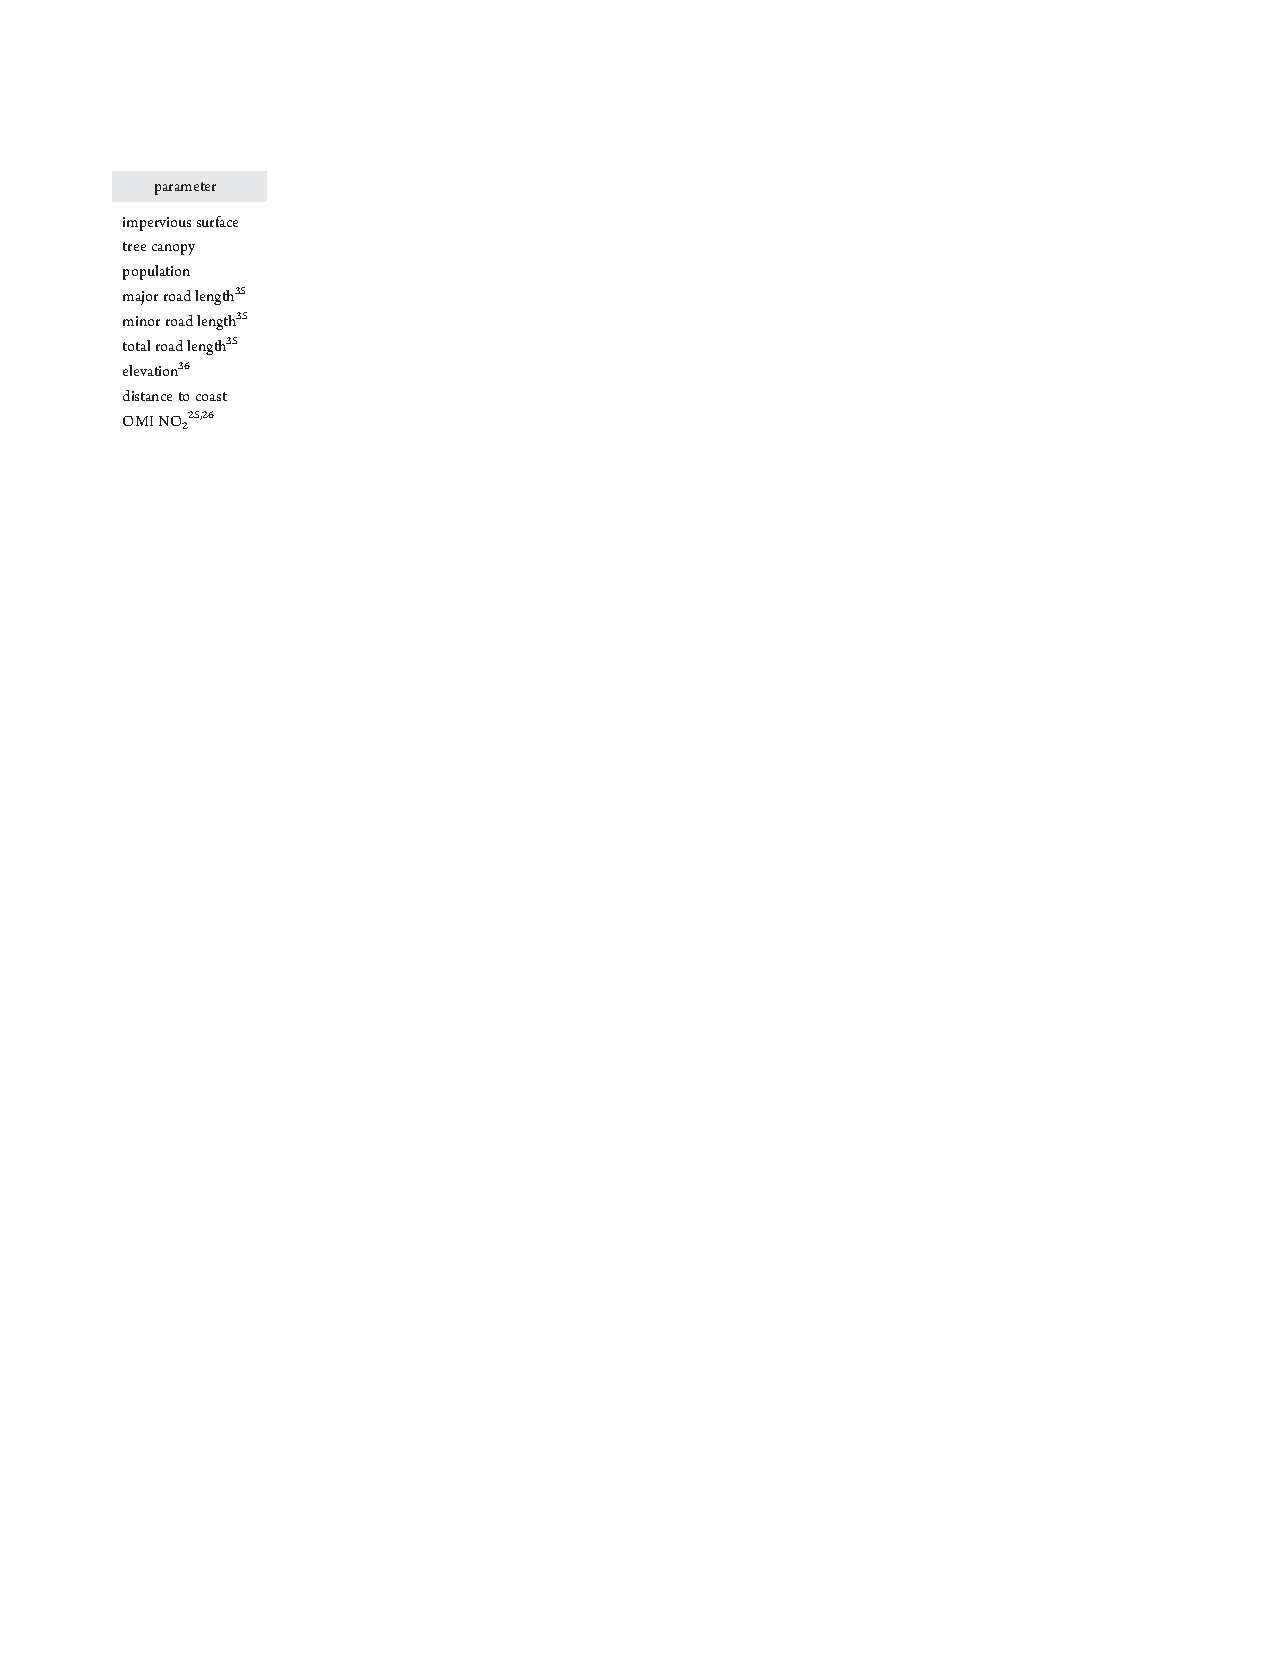
\includegraphics[height=0.6\textheight]{novotny_tab1_1}

\includegraphics[height=0.6\textheight]{novotny_tab1_2}
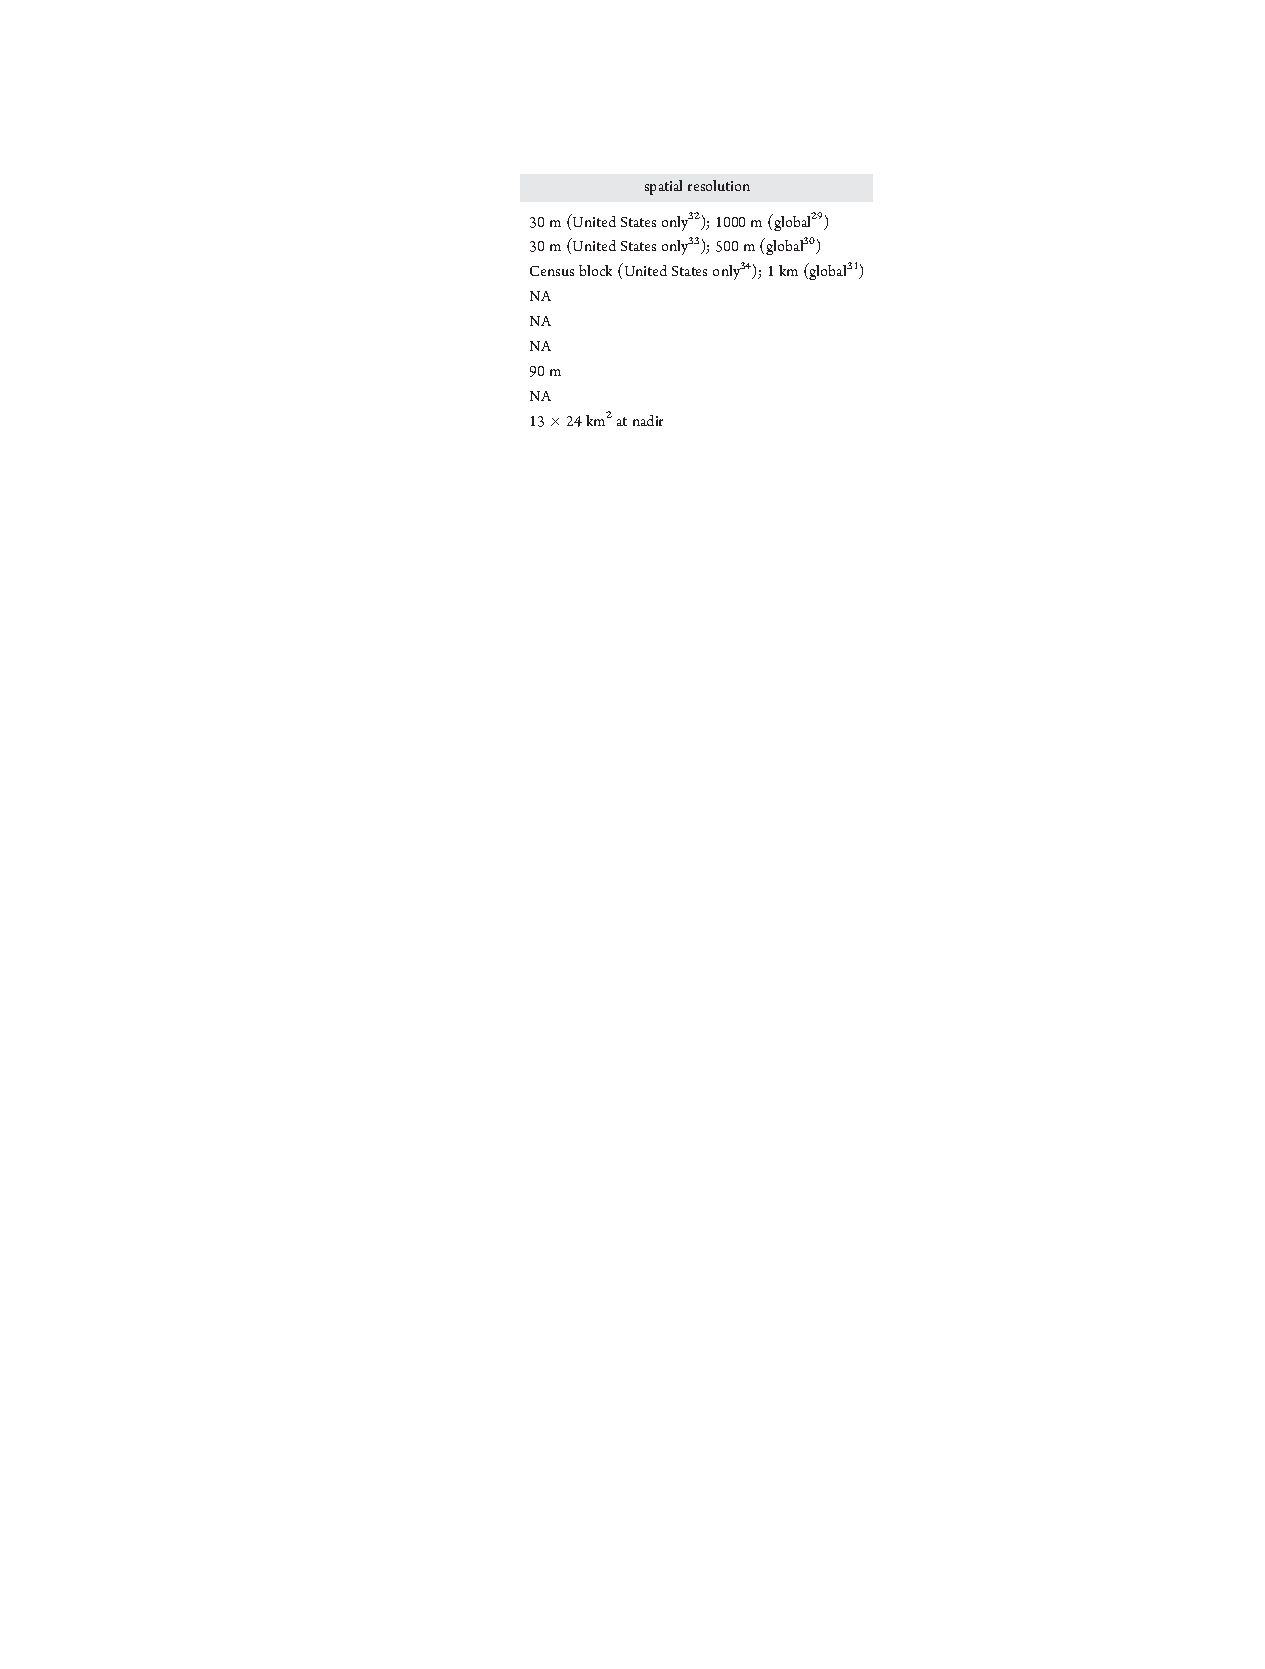
\includegraphics[height=0.6\textheight]{novotny_tab1_3}
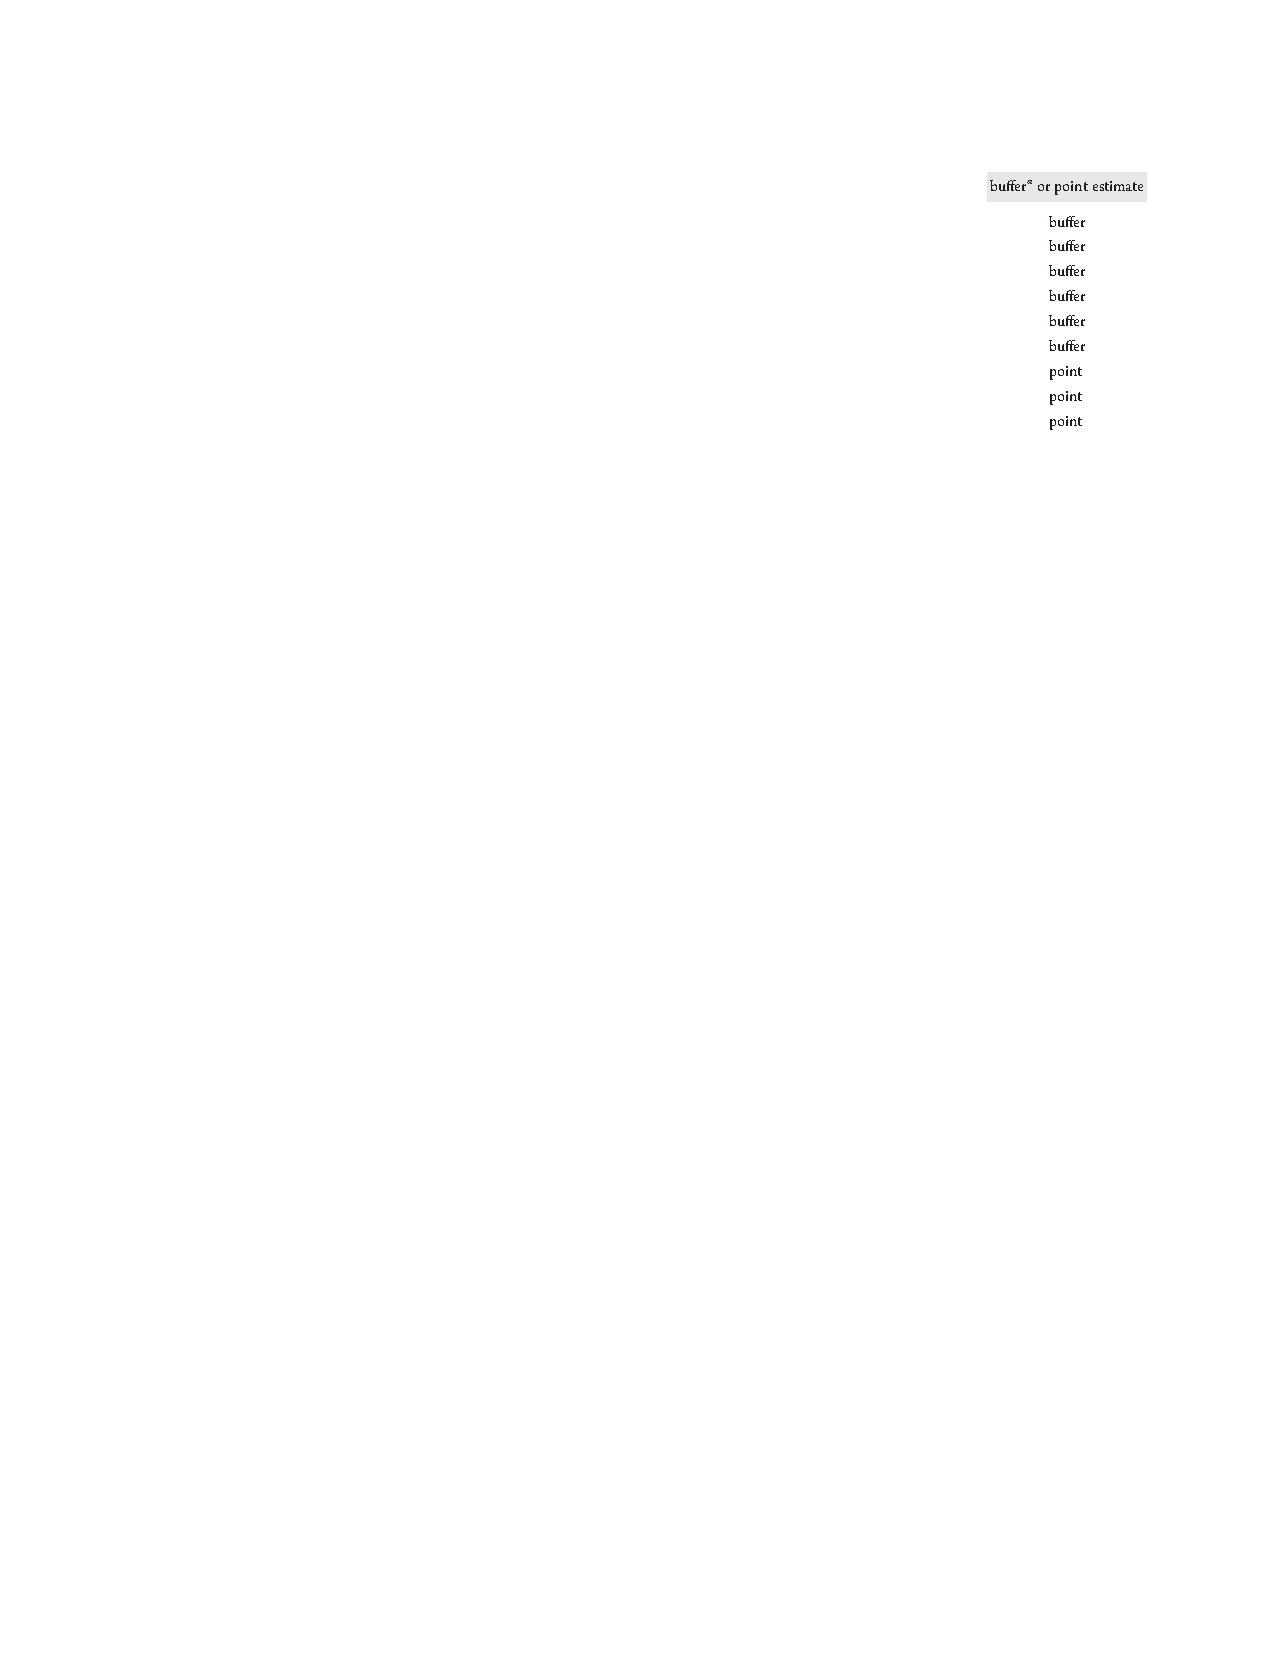
\includegraphics[height=0.6\textheight]{novotny_tab1_4}
\caption*{Novotny \textit{et al} Table 1.  }
\end{figure}

\end{frame}


\begin{frame}{}
	Let's run some linear regression models with these data.  Move over to data hub.

\end{frame}

\begin{frame}{Reading questions}

\begin{itemize}
\item  Review Figure 1 in detail.  From a visualization perspective, what features of the figure do you appreciate?  Do you think it could be improved upon?
\item In the section \textbf{Electricity and human development}, the authors state that their figure is 'consistent with an aggregate view of household-level diminishing returns on energy consumption....'  Discuss what the authors mean by this statement.  Do you agree?
\item  In the section \textbf{The electricity continuum}, the authors argue that 'By overcoming access barriers, often through market-based structures, these systems provide incremental and often substantial increases in access to services, compared with the status quo.'  Contrast this statement to the premise of Lee \textit{et al} (which we read last week).  Is Alstone \textit{et al}'s view consistent or in conflict with Lee \textit{et al}?  
\end{itemize}

\end{frame}

\begin{frame}
Supplemental
\end{frame}


\begin{frame}{Important Questions for Multiple Linear Regression}
  \begin{itemize}
    \item Is at least one of the predictors X1 , X2 , . . . , Xp useful in predicting the response?
    \begin{itemize}
      \item cover only briefly
    \end{itemize}
    \item Do all the predictors help to explain Y, or is only a subset of the predictors useful?
    \begin{itemize}
      \item Review variable selection.  
      \item Cue attention to Marshall et al approach.
    \end{itemize}
    \item How well does the model fit the data?
    \begin{itemize}
      \item Return to question of Rsq
    \end{itemize}
    \item Given a set of predictor values, what response value should we predict, and how accurate is our prediction?  
    \begin{itemize}
      \item Prediction intervals (contrast to confidence intervals)
    \end{itemize}
  \end{itemize}
\end{frame}



\begin{frame}{Basic sketch of the Novotny et al paper:}
``Stepwise multivariate regression'':
\begin{enumerate}
\item The independent variable most correlated with the dependent variable is added to the model first
\item Of the remaining variables, the one most correlated with model residuals is selected as the next independent variable
\item Step 2 repeats on each new model with the remaining variables.  
\begin{itemize}
\item Variables are not kept in the model if $p>0.05$
\item Variables are not kept in the model if they are collinear with others (we'll discuss this Tuesday).
\end{itemize}
\end{enumerate}
\end{frame}


\begin{frame}{Basic sketch for Novotny, ctd}

Choosing the model:
\begin{itemize}
\item Model-building using a random sample of 90\% of the monitoring data 
\item Tested the model's ability to predict the remaining 10\%. 
\item Create 500 different random samples of training data -- calculate R2, error, and bias for all 500 iterations. 
\end{itemize}

\textbf{Question}: Why build the model with 90\% of the data only?\pause

\vspace{5mm}
\textbf{Answer}: to avoid choosing a model that over-fits the data.

\vspace{5mm}
In HW9, we'll go through a process similar (and arguably superior) to this one.

\vspace{5mm}
In HW6 -- next week -- we'll use a different method, known as AIC.  We'll go over that today.  
\end{frame}
	
\end{document}


